%% abtex2-modelo-trabalho-academico.tex, v-1.9.2 laurocesar
%% Copyright 2012-2014 by abnTeX2 group at http://abntex2.googlecode.com/ 
%%
%% This work may be distributed and/or modified under the
%% conditions of the LaTeX Project Public License, either version 1.3
%% of this license or (at your option) any later version.
%% The latest version of this license is in
%%   http://www.latex-project.org/lppl.txt
%% and version 1.3 or later is part of all distributions of LaTeX
%% version 2005/12/01 or later.
%%
%% This work has the LPPL maintenance status `maintained'.
%% 
%% The Current Maintainer of this work is the abnTeX2 team, led
%% by Lauro César Araujo. Further information are available on 
%% http://abntex2.googlecode.com/
%%
%% This work consists of the files abntex2-modelo-trabalho-academico.tex,
%% abntex2-modelo-include-comandos and abntex2-modelo-references.bib
%%

% ------------------------------------------------------------------------
% ------------------------------------------------------------------------
% abnTeX2: Modelo de Trabalho Academico (tese de doutorado, dissertacao de
% mestrado e trabalhos monograficos em geral) em conformidade com 
% ABNT NBR 14724:2011: Informacao e documentacao - Trabalhos academicos -
% Apresentacao
% ------------------------------------------------------------------------
% ------------------------------------------------------------------------

%-------------------------------------------------------------------------
% Modelo adaptado especificamente para o contexto do PPgSI-EACH-USP por 
% Marcelo Fantinato, com auxílio dos Professores Norton T. Roman, Helton
% H. Bíscaro, e Sarajane M. Peres, em 2015, com muitos agradecimentos aos 
% criadores da classe e do modelo base.
%-------------------------------------------------------------------------

\documentclass[
	% -- opções da classe memoir --
	12pt,				% tamanho da fonte
	% openright,			% capítulos começam em pág ímpar (insere página vazia caso preciso)
	oneside,			% para impressão apenas no anverso (apenas frente). Oposto a twoside
	a4paper,			% tamanho do papel. 
	% -- opções da classe abntex2 --
	%chapter=TITLE,		% títulos de capítulos convertidos em letras maiúsculas
	%section=TITLE,		% títulos de seções convertidos em letras maiúsculas
	%subsection=TITLE,	% títulos de subseções convertidos em letras maiúsculas
	%subsubsection=TITLE,% títulos de subsubseções convertidos em letras maiúsculas
	% -- opções do pacote babel --
	english,			% idioma adicional para hifenização
	%french,				% idioma adicional para hifenização
	%spanish,			% idioma adicional para hifenização
	brazil				% o último idioma é o principal do documento
	]{abntex2ppgsi}

% ---
% Pacotes básicos 
% ---
% \usepackage{lmodern}			% Usa a fonte Latin Modern			
% \usepackage[T1]{fontenc}		% Selecao de codigos de fonte.
\usepackage[utf8]{inputenc}		% Codificacao do documento (conversão automática dos acentos)
\usepackage{lastpage}			% Usado pela Ficha catalográfica
\usepackage{indentfirst}		% Indenta o primeiro parágrafo de cada seção.
\usepackage{color}				% Controle das cores
\usepackage{graphicx}			% Inclusão de gráficos
\usepackage{microtype} 			% para melhorias de justificação
\usepackage{pdfpages}     %para incluir pdf
\usepackage{algorithm}			%para ilustrações do tipo algoritmo
\usepackage{mdwlist}			%para itens com espaço padrão da abnt
\usepackage[noend]{algpseudocode}			%para ilustrações do tipo algoritmo
\usepackage{listings}
\usepackage{amsmath}
		
% ---
% Pacotes adicionais, usados apenas no âmbito do Modelo Canônico do abnteX2
% ---
\usepackage{lipsum}				% para geração de dummy text
% ---

% ---
% Pacotes de citações
% ---
\usepackage[brazilian,hyperpageref]{backref}	 % Paginas com as citações na bibl
\usepackage[alf]{abntex2cite}	% Citações padrão ABNT

% --- 
% CONFIGURAÇÕES DE PACOTES
% --- 

% ---
% Configurações do pacote backref
% Usado sem a opção hyperpageref de backref
\renewcommand{\backrefpagesname}{Citado na(s) página(s):~}
% Texto padrão antes do número das páginas
\renewcommand{\backref}{}
% Define os textos da citação
\renewcommand*{\backrefalt}[4]{
	\ifcase #1 %
		Nenhuma citação no texto.%
	\or
		Citado na página #2.%
	\else
		Citado #1 vezes nas páginas #2.%
	\fi}%
% ---

% ---
% Informações de dados para CAPA e FOLHA DE ROSTO
% ---

%-------------------------------------------------------------------------
% Comentário adicional do PPgSI - Informações sobre o ``instituicao'':
%
% Não mexer. Deixar exatamente como está.
%
%-------------------------------------------------------------------------
\instituicao{
	UNIVERSIDADE DE SÃO PAULO
	\par
	ESCOLA DE ARTES, CIÊNCIAS E HUMANIDADES
	\par
	BACHARELADO EM SISTEMAS DE INFORMAÇÃO
        \par
        ORGANIZAÇÃO E ARQUITETURA DE COMPUTADORES I}

%-------------------------------------------------------------------------
% Comentário adicional do PPgSI - Informações sobre o ``título'':
%
% Em maiúscula apenas a primeira letra da sentença (do título), exceto 
% nomes próprios, geográficos, institucionais ou Programas ou Projetos ou 
% siglas, os quais podem ter letras em maiúscula também.
%
% O subtítulo do trabalho é opcional.
% Sem ponto final.
%
% Atenção: o título da Dissertação na versão corrigida não pode mudar. 
% Ele deve ser idêntico ao da versão original.
%
%-------------------------------------------------------------------------
\titulo{RELATÓRIO DE ORGANIZAÇÃO E ARQUITETURA DE COMPUTADORES I}

%-------------------------------------------------------------------------
% Comentário adicional do PPgSI - Informações sobre o ``autor'':
%
% Todas as letras em maiúsculas.
% Nome completo.
% Sem ponto final.
%-------------------------------------------------------------------------
\autor{\uppercase{Júlia Du Bois Araújo Silva\\MARCOS MEDEIROS DA SILVA FILHO}}

%-------------------------------------------------------------------------
% Comentário adicional do PPgSI - Informações sobre o ``local'':
%
% Não incluir o ``estado''.
% Sem ponto final.
%-------------------------------------------------------------------------
\local{São Paulo - SP}

%-------------------------------------------------------------------------
% Comentário adicional do PPgSI - Informações sobre a ``data'':
%
% Colocar o ano do depósito (ou seja, o ano da entrega) da respectiva 
% versão, seja ela a versão original (para a defesa) seja ela a versão 
% corrigida (depois da aprovação na defesa). 
%
% Atenção: Se a versão original for depositada no final do ano e a versão 
% corrigida for entregue no ano seguinte, o ano precisa ser atualizado no 
% caso da versão corrigida. 
% Cuidado, pois o ano da ``capa externa'' também precisa ser atualizado 
% nesse caso.
%
% Não incluir o dia, nem o mês.
% Sem ponto final.
%-------------------------------------------------------------------------
\data{2024}

%-------------------------------------------------------------------------
% Comentário adicional do PPgSI - Informações sobre o ``Orientador'':
%
% Se for uma professora, trocar por ``Profa. Dra.''
% Nome completo.
% Sem ponto final.
%-------------------------------------------------------------------------
\orientador{Prof. Dr. Fulano de Tal}

%-------------------------------------------------------------------------
% Comentário adicional do PPgSI - Informações sobre o ``Coorientador'':
%
% Opcional. Incluir apenas se houver co-orientador formal, de acordo com o 
% Regulamento do Programa.
%
% Se for uma professora, trocar por ``Profa. Dra.''
% Nome completo.
% Sem ponto final.
%-------------------------------------------------------------------------
\coorientador{Prof. Dr. Fulano de Tal}

\tipotrabalho{Dissertação (Mestrado)}

% ---


% ---
% Configurações de aparência do PDF final

% alterando o aspecto da cor azul
\definecolor{blue}{RGB}{41,5,195}

% informações do PDF
\makeatletter
\hypersetup{
     	%pagebackref=true,
		pdftitle={\@title}, 
		pdfauthor={\@author},
    	pdfsubject={\imprimirpreambulo},
	    pdfcreator={LaTeX com abnTeX2 adaptado para o PPgSI-EACH-USP},
		pdfkeywords={abnt}{latex}{abntex}{abntex2}{qualificação de mestrado}{dissertação de mestrado}{ppgsi}, 
		colorlinks=true,       		% false: boxed links; true: colored links
    	linkcolor=black,          	% color of internal links
    	citecolor=black,        		% color of links to bibliography
    	filecolor=black,      		% color of file links
		urlcolor=black,
		bookmarksdepth=4
}
\makeatother
% --- 

% --- 
% Espaçamentos entre linhas e parágrafos 
% --- 

% O tamanho do parágrafo é dado por:
\setlength{\parindent}{1.25cm}

% Controle do espaçamento entre um parágrafo e outro:
\setlength{\parskip}{0cm}  % tente também \onelineskip
\renewcommand{\baselinestretch}{1.5}

% ---
% compila o indice
% ---
\makeindex
% ---

	% Controlar linhas orfas e viuvas
  \clubpenalty10000
  \widowpenalty10000
  \displaywidowpenalty10000

% ----
% Início do documento
% ----
\begin{document}

% Retira espaço extra obsoleto entre as frases.
\frenchspacing 

% ----------------------------------------------------------
% ELEMENTOS PRÉ-TEXTUAIS
% ----------------------------------------------------------
% \pretextual

% ---
% Capa
% ---
%-------------------------------------------------------------------------
% Comentário adicional do PPgSI - Informações sobre a ``capa'':
%
% Esta é a ``capa'' principal/oficial do trabalho, a ser impressa apenas 
% para os casos de encadernação simples (ou seja, em ``espiral'' com 
% plástico na frente).
% 
% Não imprimir esta ``capa'' quando houver ``capa dura'' ou ``capa brochura'' 
% em que estas mesmas informações já estão presentes nela.
%
%-------------------------------------------------------------------------
\imprimircapa
% ---

% ---
% ---
% inserir o sumario
% ---
\pdfbookmark[0]{\contentsname}{toc}
\tableofcontents*
\cleardoublepage
% ---



% ----------------------------------------------------------
% ELEMENTOS TEXTUAIS
% ----------------------------------------------------------
\textual



%-------------------------------------------------------------------------
% Comentário adicional do PPgSI - Informações sobre ``títulos de seções''
% 
% Para todos os títulos (seções, subseções, tabelas, ilustrações, etc):
%
% Em maiúscula apenas a primeira letra da sentença (do título), exceto 
% nomes próprios, geográficos, institucionais ou Programas ou Projetos ou
% siglas, os quais podem ter letras em maiúscula também.
%
%-------------------------------------------------------------------------
\chapter{Organização e arquitetura MIPS}
\textbf{Assembly} é uma linguagem de máquina que possui mecanismos para nomear padrões de bits que ocorrem comumente, como opcodes e especificadores de registradores, e permite que os programadores utilizem rótulos para identificar e nomear partes particulares da memória que mantêm instruções ou dados. 

\section{Memória}
Os sistemas baseados em MIPS, em sua maioria, dividem a memória em três partes, ilustradas na imagem seguinte:

\begin{figure}[h]
    \centering
    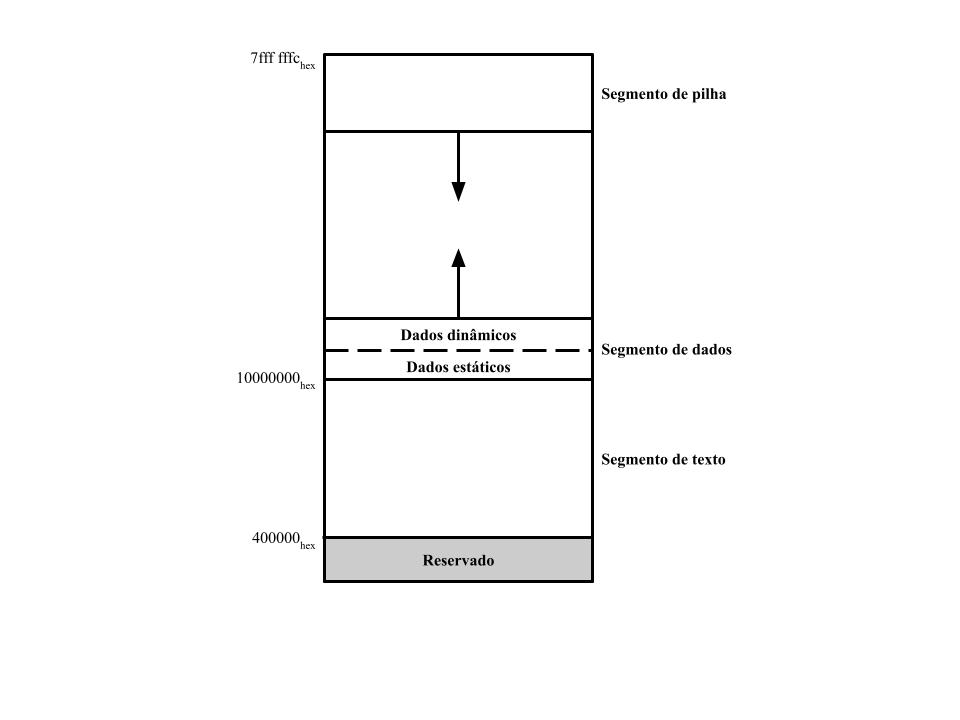
\includegraphics[width=17cm]{memoriaMIPS.jpg}
    \caption{Layout da memória da maioria dos programas baseados em MIPS}
    \label{fig:enter-label}
\end{figure}

Essas partes são:

\begin{itemize}
    \item \textbf{Segmento de pilha}: reside no topo do espaço de endereçamento virtual e não tem um tamanho máximo definido previamente. Essa parte da memória é utilizada por um programa para manter frames de chamada de procedimento e expande para baixo na direção do segmento de dados.
    \item \textbf{Segmento de dados}: parte central da memória, dividida internamente em duas partes:
        \begin{itemize}
            \item \textbf{Dados dinâmicos}: parte inferior do segmento de dados, contendo objetos cujo tamanho é conhecido pelo compilador e cujo tempo de vida corresponde ao tempo de execução inteira do programa. Objetos estáticos são atribuidos a locais no segmento de dados pelo link-editor, o qual também resolve referências a esses objetos.
            \item \textbf{Dados estáticos}: parte superior do segmento de dados, responsável pelos dados alocados no decorrer da execução de um programa. Essa área é expandida para cima, na direção do segmento de pilha, de acordo com a demanda necessária. 
        \end{itemize}
    \item \textbf{Segmento de texto}: parte inferior da memória, a qual mantém as instruções do programa.
\end{itemize}

Essa organização, embora não obrigatória, possui duas características importantes: a grande distância entre os dois segmentos dinamicamente expansíveis e o fato de que esses segmentos podem crescer para ocupar o espaço de endereços completo de um programa.

\section{Registradores}
A CPU do MIPS contém 32 registradores de uso geral, numerados de 0 a 31. Esses registradores possuem nomes e usos como descritos na Tabela 1.

\begin{table}[h]
    \centering
    \begin{tabular}{c|c|l}
        Nome & Número & Uso \\ \hline
        \$zero & 0 & constante 0\\ \hline
        \$at & 1 & reservado para o montador\\ \hline
        \$v0 & 2 & avaliação de expressão e resultados de uma função\\ \hline
        \$v1 & 3 & avaliação de expressão e resultados de uma função\\ \hline
        \$a0 & 4 & argumento 1\\ \hline
        \$a1 & 5 & argumento 2\\ \hline
        \$a2 & 6 & argumento 3\\ \hline
        \$a3 & 7 & argumento 4\\ \hline
        \$t0 & 8 & temporário (não preservado pela chamada)\\ \hline
        \$t1 & 9 & temporário (não preservado pela chamada)\\ \hline
        \$t2 & 10 & temporário (não preservado pela chamada)\\ \hline
        \$t3 & 11 & temporário (não preservado pela chamada)\\ \hline
        \$t4 & 12 & temporário (não preservado pela chamada)\\ \hline
        \$t5 & 13 & temporário (não preservado pela chamada)\\ \hline
        \$t6 & 14 & temporário (não preservado pela chamada)\\ \hline
        \$t7 & 15 & temporário (não preservado pela chamada)\\ \hline
        \$s0 & 16 & temporário salvo (preservado pela chamada)\\ \hline
        \$s1 & 17 & temporário salvo (preservado pela chamada)\\ \hline
        \$s2 & 18 & temporário salvo (preservado pela chamada)\\ \hline
        \$s3 & 19 & temporário salvo (preservado pela chamada)\\ \hline
        \$s4 & 20 & temporário salvo (preservado pela chamada)\\ \hline
        \$s5 & 21 & temporário salvo (preservado pela chamada)\\ \hline
        \$s6 & 22 & temporário salvo (preservado pela chamada)\\ \hline
        \$s7 & 23 & temporário salvo (preservado pela chamada)\\ \hline
        \$t8 & 24 & temporário (não preservado pela chamada)\\ \hline
        \$t9 & 25 & temporário (não preservado pela chamada)\\ \hline
        \$k0 & 26 & reservado para o kernel do sistema operacional\\ \hline
        \$k1 & 27 & reservado para o kernel do sistema operacional\\ \hline
        \$gp & 28 & ponteiro para área global\\ \hline
        \$sp & 29 & stack pointer\\ \hline
        \$fp & 30 & frame pointer\\ \hline
        \$ra & 31 & endereço de retorno (usado por chamada de função)\\ \hline\end{tabular}
    \caption{Registradores do MIPS e convenção de uso}
    \label{tabRegistradores}
\end{table}

\section{Tratamento de exceções}

Nos processadores MIPS, uma parte da CPU chamada de co-processador 0 é responsável pelo registro das informações necessárias para lidar com exceções e interrupções. Exceções e interrupções fazem com que um processador MIPS desvie para uma parte do código, no endereço $80000180_{\text{hexa}}$ (no espaço de endereçamento do kernel, não do usuário), chamada \textbf{handler de exceção}.

\section{Modos de endereçamento}

O MIPS é uma arquitetura \textit{load store}, ou seja, apenas as instruções \textit{load} e \textit{store} podem acessar a memória e as instruções de cálculo operam apenas sobre os valores dos registradores. A máquina virtual oferece os seguintes modos de endereçamento para intruções \textit{load} e \textit{store}: 

\begin{figure}[h]
    \centering
    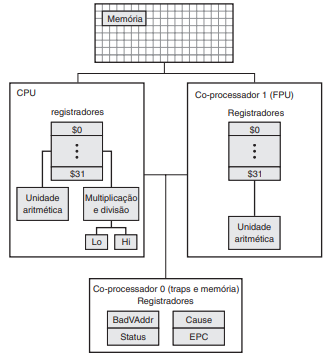
\includegraphics[width=0.75\linewidth]{modosEnd1.png}
    \caption{CPU e FPU do MIPS R2000}
    \label{figModEnd1}
\end{figure}

\section{Opcode}

Cada instrução MIPS é codificada em um número binário, de acordo com a codificação de instruções para um campo a partir de uma instrução. A figura a seguir explicada como uma instrução é codificada:

\begin{figure}[h]
    \centering
    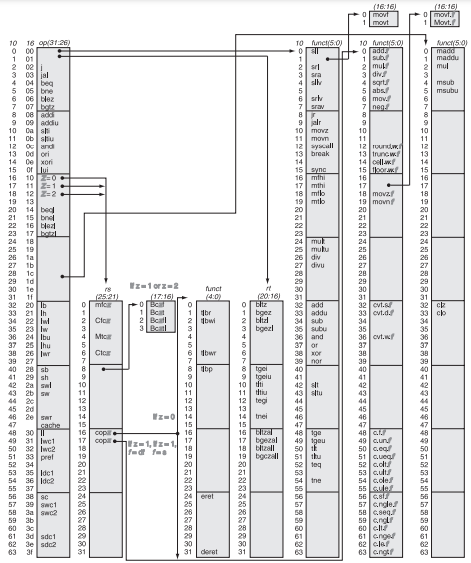
\includegraphics[width=1\linewidth]{opcodes.png}
    \caption{Mapa de opcode do MIPS}
    \label{figOpcode}
\end{figure}

\chapter{Descrição do problema e código alto nível da solução}
Para entregar o trabalho e obter uma maior compreensão sobre a linguagem de montagem MIPS, foram desenvolvidas as soluções dos itens A, B e C do problema 27 \cite{temp1}:

\begin{itemize}
    \item[A.] Faça uma função que recebe como parâmetros um inteiro  e duas matrizes quadradas reais $X$ e $Y$ de ordem $n$. Esta função devolve em uma matriz $Z$, também passada como parâmetro, a soma das matrizes $X$ e $Y$;
    \item[B.] Escreva uma função que recebe como parâmetro um número inteiro $n$, um número real $c$ e uma matriz $X_{n \times n}$. A função devolve em uma matriz $Y$, também passada como parâmetro, o produto do número $c$ pela matriz $X$. Ou seja, $Y_{ij}=c \times X_{ij}$ para $0<i<n-1$ e $0<j<n-1$;
    \item[C.] Escreva uma função que recebe como parâmetros um inteiro $n$ e duas matrizes quadradas reais $X_{n \times n}$ e $Y_{n \times n}$. Esta função devolve em uma matriz $Z$, também passada como parâmetro, o produto das matrizes $X$ e $Y$.
    
\end{itemize}

Nesse sentido, o item A solicita que se desenvolva uma função, o qual recebe como parâmetros um inteiro $n$, que representa a dimensão da matriz quadrada real $M_{n \times n}$, dois ponteiros para as matrizes reais $X_{n \times n}$ e $Y_{n \times n}$ e um ponteiro que receberá uma matriz quadrada real $Z_{n \times n}$ resultante da operação da função. Sob essa ótica, a função realizará a operação de soma entre as matrizes $X_{n \times n}$ e $Y_{n \times n}$ e atribuirá a matriz resultante no ponteiro passado como parâmetro, ou seja, $Z_{n \times n}=X_{n \times n} + Y_{n \times n}$.

Com isso, foi desenvolvido tal função utilizando a linguagem C, o qual se chama “addMatriz”, em que se realiza a operação descrita anteriormente e retorna um valor lógico, sinalizando se foi possível efetuar a procedimento. Conforme visto na imagem abaixo, verifica-se se foi passado uma dimensão $n$ válida para realizar a operação, aloca-se dinamicamente uma matriz $Z_{n \times n}$ ao ponteiro passado como parâmetro e posteriormente se realiza a soma $Z_{ij}=X_{ij}+Y_{ij}$ através de uma estrutura de repetição duplamente encadeada com $0<i<n$ e $0<j<n$. Após isso, retorna-se verdadeiro se a condição inicial for falsa, senão se retorna falso sinalizando que não é possível realizar a soma com dimensão inválida.

\begin{lstlisting}[language=C, caption=Resolução de alto nível do exercício 27.A]
bool addMatriz(int n, double*** x, double*** y, double*** z){
    if(n < 2) return false;
    *z = (double**) malloc(sizeof(double*)*n);
    for(int i = 0; i < n; i++){
        (*z)[i] = (double*) malloc(sizeof(double) * n);
    }
    for(int i = 0; i < n; i++){
        for(int j = 0; j < n; j++){
            (*z)[i][j] = (*x)[i][j] + (*y)[i][j];
        }
    }

    return true;
}
\end{lstlisting}

Ademais, o item B solicita que se produza uma função, o qual recebe como parâmetros um inteiro $n$, que representa a dimensão da matriz quadrada real $M_{n \times n}$, um ponteiro para a matriz real $X_{n \times n}$, uma constante $c$ real e um ponteiro que receberá uma matriz quadrada real $Y_{n \times n}$ resultante da operação da função. Nesse viés, a função multiplicará a matriz  pela constante $c$ e atribuirá a matriz resultante no ponteiro passado como parâmetro, ou seja, $Y_{n \times n}= X_{n \times n} \cdot c$.

Assim, foi feita a função do item B com a linguagem C, o qual se denomina “mulConstMatriz”, em que se realiza a operação descrita anteriormente e retorna um valor lógico, sinalizando se foi possível efetuar a procedimento. Conforme visto na imagem abaixo, verifica-se se foi passado uma dimensão $n$ válida para realizar a operação, aloca-se dinamicamente uma matriz $Y_{n \times n}$ ao ponteiro passado como parâmetro e posteriormente se realiza a multiplicação $Y_{ij}=X_{ij} \cdot c$ através de uma estrutura de repetição duplamente encadeada com $0<i<n$ e $0<j<n$. Após isso, retorna-se verdadeiro se a condição inicial for falsa, senão se retorna falso sinalizando que não é possível realizar a multiplicação com dimensão inválida.

\begin{lstlisting}[language=C, caption=Resolução de alto nível do exercício 27.B]
bool mulConstMatriz(int n, double c, double*** x, double*** y){
    if(n < 2) return false;
    *y = (double**) malloc(sizeof(double*)*n);
    for(int i = 0; i < n; i++){
        (*y)[i] = (double*) malloc(sizeof(double)*n);
    }
    for(int i = 0; i < n; i++){
        for(int j = 0; j < n; j++){
            (*y)[i][j] = c * (*x)[i][j];
        }
    }
    
    return true;
}
\end{lstlisting}

Outrossim, o item C solicita que se produza uma função, o qual recebe como parâmetros um inteiro n, que representa a dimensão da matriz quadrada real $M_{n \times n}$, dois ponteiros para as matrizes reais $X_{n \times n}$ e $Y_{n \times n}$ e um ponteiro que receberá uma matriz quadrada real $Z_{n \times n}$ resultante da operação da função. Nesse viés, a função multiplicará a matriz  pela matriz  e atribuirá a matriz resultante no ponteiro passado como parâmetro, ou seja, $Z_{n \times n} = X_{n \times n} \cdot Y_{n \times n}$.

Dessa forma, foi efetuada a função do item C com a linguagem C, o qual se denomina “mulMatriz”, em que se realiza a operação descrita anteriormente e retorna um valor lógico, sinalizando se foi possível efetuar a procedimento.  Consoante a imagem abaixo, verifica-se se foi passado uma dimensão  válida para realizar a operação, aloca-se dinamicamente uma matriz $Z_{n \times n}$ ao ponteiro passado como parâmetro, inicializa a matriz alocada com valor zero e posteriormente se realiza a operação $Z_{ij}= \sum_{k=0}^{n}X_{ik}\times Y_{kj}$, 	que é a soma do valor anterior de $Z_{ij}$ e o produto e, posteriormente, a atribuição deste resultado a $Z_{ij}$, através de uma estrutura de repetição triplamente encadeada com $i, j \text{e} k \in $. Com isso, obtém-se $Z_{n \times n}=X_{n\ \times n} \cdot Y_{n \times n}$ e, assim, retorna-se verdadeiro se a condição inicial for falsa, senão se retorna falso sinalizando que não é possível realizar a multiplicação com dimensão inválida.

\begin{lstlisting}[language=C, caption=Resolução de alto nível do exercício 27.C]
bool mulMatriz(int n, double*** x, double*** y, double*** z){
    if(n < 2) return false;
    *z = (double**) malloc(sizeof(double*)*n);
    for(int i = 0; i < n; i++){
        (*z)[i] = (double*) malloc(sizeof(double)*n);
        for(int j = 0; j < n; j++) (*z)[i][j] = 0;
    }
    for(int i = 0; i < n; i++){
        for(int j = 0; j < n; j++){
            for(int k = 0; k < n; k++){
                (*z)[i][j] += (*x)[i][k]*(*y)[k][j];
            }
        }
    }

    return true;
}
\end{lstlisting}

\chapter{Código em Assembly desenvolvido}

O montador utilizado nesse trabalho é o MARS (MIPS Assembler and Runtime Simulator), desenvolvido e mantido pela Missouri State University.

\section{Exercício 27.A}
\begin{lstlisting}[language={[x86masm]Assembler}, caption=Resolução em baixo nível do exercício 27.A]
.data
    ## Mensagem de erro:
    error: .asciiz "Nao eh possivel realizar a operacao"
    
    ## Matrizes:
    m1: .double 4.0, 4.0, 4.0, 4.0, 4.0, 4.0, 4.0, 4.0, 4.0
    m2: .double 4.0, 4.0, 4.0, 4.0, 4.0, 4.0, 4.0, 4.0, 4.0

    ## Dimensao da matriz:
    n: .word 3

    ## Tamanho de um double
    dbl_size: .word 8
    
    format: .asciiz " "
    newline: .asciiz "\n"
    
.text
.globl main
main:
addMatriz:
    lw $t1, n   ## Carrega a dimensao n das matrizes
    blt $t1, 2, exception
        ##Se matriz invalida, nao executa procedimento
    lw $t2, dbl_size    ## Carrega o tamanho do double
    mul $t3, $t1, $t1   ## (n*n)
    mul $t3, $t3, $t2   ## (n*n)*dbl_size
    jal alocation   ## Aloca dinamicamente a matriz resultante
    li $s0, 0   ## i = 0
    li $s1, 0   ## j = 0
    la $a0, m1  ## Enderenco base da matriz M1
    la $a1, m2
    L1:
        li $s1, 0	
        L2:
            mul $t5, $s0, $t1   ## i*n
            addu $t5, $t5, $s1  ## (i*n) + j
            mul $t5, $t5, $t2   ## [(i*n) + j]*dbl_size
            addu $t6, $a0, $t5  ## m1[i][j]
            addu $t7, $a1, $t5  ## m2[i][j]
            l.d $f2, ($t6)
            l.d $f4, ($t7)
            add.d $f2, $f2, $f4 ## m1[i][j] + m2[i][j]
            addu $t6, $t4, $t5  ## x[i][j]
            s.d $f2, ($t6)  ## x[i][j] = m1[i][j] + m2[i][j]
            addi $s1, $s1, 1
            blt $s1, $t1, L2    ## se j < n, repita o processo
        addi $s0, $s0, 1
        blt $s0, $t1, L1    ## se x < n, repita o processo
    jal print     ## imprime a matriz x
    j end

print:
    li $s0, 0
    li $s1, 0
    addi $sp, $sp, -4 ## desloca o armazenamento necessario na pilha
    sw $ra, ($sp) ## armazena o endereco de retorno na pilha
    K1:
        li $s1, 0	
        K2:
            mul $t5, $s0, $t1
            addu $t5, $t5, $s1
            mul $t5, $t5, $t2
            addu $t6, $t4, $t5
            l.d $f12, ($t6)
            li $v0, 3   ## imprime x[i][j]
            syscall
            la $a0, format
            li $v0, 4   ## imprime espacamento
            syscall
            addi $s1, $s1, 1
            blt $s1, $t1, K2
            jal nextline    ## imprime \n
        addi $s0, $s0, 1
        blt $s0, $t1, K1
    lw $ra, ($sp)   ## devolve o endereco de retorno
    addi $sp, $sp, 4
    jr $ra

nextline:
    addi $sp, $sp, -4
    sw $ra, ($sp)
    la $a0, newline
    li $v0, 4   ## imprime \n
    syscall
    lw $ra, ($sp)
    addi $sp, $sp, 4
    jr $ra

alocation:
    addi $sp, $sp, -4
    sw $ra, ($sp)
    li $v0, 9   ## aloca matriz x dinamicamente
    move $a0, $t3   ## matriz com n*n elementos
    syscall
    move $t4, $v0   ## transfere o endereco base da matriz x
    lw $ra, ($sp)
    addi $sp, $sp, 4
    jr $ra

end:
    li $v0, 10  ## encerra o programa
    syscall	

exception:
    la $a0, error
    li $v0, 4 ## exibe mensagem de erro
    syscall
    j end				
\end{lstlisting}

\section{Exercício 27.B}
\begin{lstlisting}[language={[x86masm]Assembler}, caption=Resolução em baixo nível do exercício 27.B]
.data
    ## Mensagem de erro	
    error: .asciiz "Nao eh possivel realizar a operacao"		

    ## Constante da multiplicacaoo
    fator: .double 3.0

    ## Matriz teste NxN
    m1: .double 4.0, 4.0, 4.0, 4.0, 4.0, 4.0, 4.0, 4.0, 4.0

    ## Dimensao da matriz
    n: .word 3

    ## Tamanho de um double
    dbl_size: .word 8
    
    format: .asciiz " "
    newline: .asciiz "\n"

.text
.globl main
main:
addMatriz:
    lw $t1, n  ## Carrega a dimensao n das matrizes
    blt $t1, 2, exception 
        ## Se matriz invalida, nao executa procedimento
    lw $t2, dbl_size    ## Carrega o tamanho do double
    mul $t3, $t1, $t1  ## (n*n)
    mul $t3, $t3, $t2  ## (n*n)*dbl_size
    jal alocation	 ## Aloca dinamicamente a matriz resultante
    li $s0, 0			## i = 0
    li $s1, 0			## j = 0
    la $a0, m1			## Enderenco base da matriz M1
    l.d $f4, fator			## Carrega o valor de c
    L1:
        li $s1, 0	
        L2:
            mul $t5, $s0, $t1		## i*n
            addu $t5, $t5, $s1	## (i*n) + j
            mul $t5, $t5, $t2 	## [(i*n) + j]*dbl_size
            addu $t6, $a0, $t5	## m1[i][j]
            l.d $f2, ($t6)
            mul.d $f2, $f2, $f4	## m1[i][j] * c
            addu $t6, $t4, $t5 	## x[i][j]
            s.d $f2, ($t6)  ## x[i][j] = m1[i][j] * c
            addi $s1, $s1, 1
            blt $s1, $t1, L2	## se j < n, repita o processo
        addi $s0, $s0, 1
        blt $s0, $t1, L1    ## se x < n, repita o processo
    jal print   ## imprime a matriz x
    j end

print:
    li $s0, 0
    li $s1, 0
    addi $sp, $sp, -4   ## desloca o armazenamento necessario na pilha
    sw $ra, ($sp)  ## armazena o endereco de retorno na pilha
    K1:
        li $s1, 0	
        K2:
            mul $t5, $s0, $t1
            addu $t5, $t5, $s1
            mul $t5, $t5, $t2
            addu $t6, $t4, $t5
            l.d $f12, ($t6)
            li $v0, 3   ## imprime x[i][j]
            syscall
            la $a0, format
            li $v0, 4   ## imprime espacamento
            syscall
            addi $s1, $s1, 1
            blt $s1, $t1, K2
        jal nextline    ## imprime \n
        addi $s0, $s0, 1
        blt $s0, $t1, K1
    lw $ra, ($sp)   ## devolve o endereco de retorno
    addi $sp, $sp, 4
    jr $ra

nextline:
    addi $sp, $sp, -4
    sw $ra, ($sp)
    la $a0, newline
    li $v0, 4   ##imprime \n
    syscall
    lw $ra, ($sp)
    addi $sp, $sp, 4
    jr $ra
	
alocation:
    addi $sp, $sp, -4
    sw $ra, ($sp)
    li $v0, 9   ## aloca matriz x dinamicamente
    move $a0, $t3   ## matriz com n*n elementos
    syscall
    move $t4, $v0	## transfere o endereco base da matriz x
    lw $ra, ($sp)
    addi $sp, $sp, 4
    jr $ra

end:
    li $v0, 10	## encerra o programa
    syscall	

exception:
    la $a0, error
    li $v0, 4	## exibe mensagem de erro
    syscall
    j end		
\end{lstlisting}

\section{Exercício 27.C}
\begin{lstlisting}[language={[x86masm]Assembler}, caption=Resolução em baixo nível do exercício 27.C]
.data
    ## Mensagem de erro
    error: .asciiz "Nao eh possivel realizar a operacao"
	
    ## Matrizes:
    m1: .double 2.0, 2.0, 2.0, 2.0, 2.0, 2.0, 2.0, 2.0, 2.0
    m2: .double 2.0, 2.0, 2.0, 2.0, 2.0, 2.0, 2.0, 2.0, 2.0
    
    zero: .double 0.0 ## auxiliar zero
    
    n: .word 3 ## dimensao da matriz
    
    dbl_size: .word 8 ## tamanho double
    
    format: .asciiz " "
    newline: .asciiz "\n"

.text
.globl main
main:
mulMatriz:
    lw $t1, n ## Carrega a dimensao da matriz
    blt $t1, 2, exception ## Se matriz invalida, encerra o programa
    lw $t2, dbl_size ## Carrega o tamanho double
    mul $t3, $t1, $t1 ## (n*n)
    mul $t3, $t3, $t2 ## (n*n)*dbl_size
    jal alocation ##aloca matriz dinamicamente
    li $s0, 0 ## i = 0
    li $s1, 0 ## j = 0 
    la $a0, m1 ## endereco base da matriz m1
    la $a1, m2
    ##inicializa a matriz
    jal fillZero
    li $s0, 0 # i = 0
    li $s1, 0 # j = 0
    li $s2, 0 # k = 0
    L1:
        li $s1, 0
        L2:
            mul $t5, $s0, $t1
            addu $t5, $s1, $t5
            mul $t5, $t5, $t2
            addu $t6, $t4, $t5 ##x[i][j]
            li $s2, 0
            L3:
                mul $t5, $s0, $t1 ## (i*n)
                addu $t5, $s2, $t5 ## (i*n) + k
                mul $t5, $t5, $t2
                addu $t7, $a0, $t5 ## m1[i][k]
                mul $t5, $s2, $t1 ## (k*n)
                addu $t5, $s1, $t5 ## (k*n) + j
                mul $t5, $t5, $t2
                addu $t8, $a1, $t5 ## m2[k][j]
                l.d $f2, ($t7)
                l.d $f4, ($t8)
                mul.d $f2, $f2, $f4 ## m1[i][k]*m2[k][j]
                l.d $f4, ($t6)
                add.d $f2, $f2, $f4 ## x[i][j] += m1[i][k]*m2[k][j]
                s.d $f2, ($t6)
                addi $s2, $s2, 1
                blt $s2, $t1, L3 ## se k < n
            addi $s1, $s1, 1
            blt $s1, $t1, L2 ## se j < n
        addi $s0, $s0, 1
        blt $s0, $t1, L1 ## se i < n
    jal print ##imprime a matriz x
    j end ## finaliza o programa
	 
fillZero:
    ##inicializa matriz x
    addi $sp, $sp, -4
    sw $ra, ($sp)
    li $s0, 0
    li $s1, 0
    S1:
        li $s1, 0
        S2:
            mul $t5, $s0, $t1 ## (i*n)
            addu $t5, $s1, $t5 ## (i*n) + j
            mul $t5, $t5, $t2 ## [(i*n) +j]*dbl_size
            addu $t6, $t4, $t5 ## x[i][j]
            la $t8, zero
            l.d $f2, ($t8)
            s.d $f2, ($t6) ## x[i][j] = 0
            addi $s1, $s1, 1
            blt $s1, $t1, S2 ## se j < n, repita o procedimento
        addi $s0, $s0, 1
        blt $s0, $t1, S1 ## se i < n, repita o procedimento
    lw $ra, ($sp)
    addi $sp, $sp, 4
    jr $ra	     	

print:
    li $s0, 0
    li $s1, 0
    addi $sp, $sp, -4 ##desloca o armazenamento necessario na pilha
    sw $ra, ($sp) ##armazena o endereco de retorno na pilha
    K1:
        li $s1, 0	
        K2:
            mul $t5, $s0, $t1
            addu $t5, $t5, $s1
            mul $t5, $t5, $t2
            addu $t6, $t4, $t5
            l.d $f12, ($t6)
            li $v0, 3 ##imprime x[i][j]
            syscall
            la $a0, format
            li $v0, 4 ##imprime espacamento
            syscall
            addi $s1, $s1, 1
            blt $s1, $t1, K2
            jal nextline ##imprime \n
        addi $s0, $s0, 1
        blt $s0, $t1, K1
    lw $ra, ($sp) ##devolve o endereco de retorno
    addi $sp, $sp, 4
    jr $ra

nextline:
    addi $sp, $sp, -4
    sw $ra, ($sp)
    la $a0, newline
    li $v0, 4 ##imprime \n
    syscall
    lw $ra, ($sp)
    addi $sp, $sp, 4
    jr $ra
	
alocation:
    addi $sp, $sp, -4
    sw $ra, ($sp)
    li $v0, 9 ##aloca matriz x dinamicamente
    move $a0, $t3 ## matriz com n*n elementos
    syscall
    move $t4, $v0 ##transfere o endereco base da matriz x
    lw $ra, ($sp)
    addi $sp, $sp, 4
    jr $ra

end:
    li $v0, 10 ##encerra o programa
    syscall	

exception:
    la $a0, error
    li $v0, 4 ## exibe mensagem de erro
    syscall
    j end			
\end{lstlisting}

\chapter{Explicação detalhada das instruções utilizadas no código}
As instruções utilizadas da arquitetura MIPS para desenvolver os programas em Assembly, considerando o nível de detalhe em micro-operações, foram as seguintes:

\begin{itemize}
    \item blt \$t1, 2, exception: é uma pseudoinstrução que verifica se o valor do registrador é menor que o número passado e, em caso verdadeiro, se desvia para a label, senão continua para a instrução seguinte. Nesse caso, é uma pseudoinstrução com valor imediato.
    \item lw \$t1, n: é uma instrução que carrega uma palavra (word) de 32 bits do endereço n ao registrador t1.
    \item mul \$t3, \$t1, \$t1: é uma instrução que realiza a multiplicação entre os últimos registradores da instrução e atribui o resultado ao registrador t3.
    \item jal multiplication: é uma instrução que realiza o desvio incondicional à label multiplication e guarda o endereço contido em program counter no registrador ra (return address).
    \item li \$s0, 0: é uma pseudoinstrução que atribui o valor imediato ao registrador passado.
    \item la \$a0, m1: é uma pseudoinstrução que carrega o endereço de memória m1 para o registrador.
    \item addu \$t6, \$a0, \$t5: é uma instrução que soma os valores sem sinal dos registradores a0 e t5 e atribui o resultado ao registrador t6.
    \item l.d \$f2, (\$t6): é uma pseudoinstrução que carrega o valor de ponto flutuante com precisão dupla ao registrador f2.
    \item add.d \$f2, \$f2, \$f4: é uma instrução que soma os valores double dos registradores f2 e f4 e atribui o resultado ao registrador f2
    \item s.d \$f2, (\$t6): é uma pseudoinstrução que armazena o double no endereço do registrador t6 no registrador f2
    \item addi \$s0, \$s0, 1: é uma instrução que soma o valor do registrador s0 com 1 e atribui o resultado a s0
    \item j end: muda o registrador PC (program counter) para o valor do label end
    \item sw \$ra, (\$sp): guarda a word do registrador ra no endereço do registrados sp 
    \item syscall: causa uma system call exception que o sistema operacional recebe e trata
    \item jr \$ra: vai incondicionalmente para a instrução cujo endereço está no registrador ra
    \item move \$t4, \$v0: move o conteúdo do registrador v0 para o registrador t4 
    \item mul.d \$f2, \$f2, \$f4: é uma instrução que multiplica o valor double dos registradores f2 e f4 e atribui o resultado ao registrador f2
\end{itemize}

Essas instruções serão detalhadas nas subseções à seguir.

\section{Instrução blt \$t1, 2, exception}
Primeiramente, branch if less than (blt) é uma pseudoinstrução, ou seja, não é uma instrução nativa do repertório da arquitetura MIPS. Dessa forma, o assembler traduz a pseudoinstrução blt para uma combinação de instruções entre slt (Set on Less Than), bne (Branch if Not Equal) e a pseudoinstrução li (Load Immediate), no caso de blt com valor imediato. No caso do li, é feita a conversão para as instruções lui (Load Upper Immediate) e ori (OR Immediate) ou para addiu (Add Immediate Unsigned), caso o valor imediato seja de 32 bits ou 16 bits, respectivamente. Assim, a execução do blt imediato com valor 2 equivale à equação sequencial do addiu, slt e bne, respectivamente.

Então, as micro-operações envolvidas e o formato em cada instrução são:

\begin{itemize}
    \item addiu \$at, \$zero, 2
    \begin{figure}[h] \centering 
\includegraphics{411.png} \caption{Formato da instrução addiu} \label{fig411} \end{figure}
    \begin{itemize}
        \item Ciclo de Busca:

            A1: MAR $\leftarrow$ PC;

            A2: MBR $\leftarrow$ Memory

            PC $\leftarrow$ PC + 4;

            A3: IR $\leftarrow$ MBR;
        \item Não há ciclo indireto
        \item Ciclo de execução:

            A1: RT $\leftarrow$ (RS) + IR(imm)
    \end{itemize}
    \item slt \$at, \$t1, \$at
    \begin{figure}[h]
        \centering
        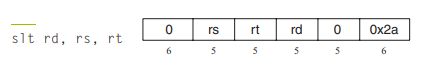
\includegraphics{412.png}
        \caption{Formato da instrução slt}
        \label{fig412}
    \end{figure}
    \begin{itemize}
        \item Ciclo de Busca:

            A1: MAR $\leftarrow$ PC;

            A2: MBR $\leftarrow$ Memory

            PC $\leftarrow$ PC + 4;

            A3: IR $\leftarrow$ MBR

        \item Não há ciclo indireto
        \item Ciclo de execução:

            A1: if(RS < RT) then RD $\leftarrow$ 1

            else RD $\leftarrow$ 0;
    \end{itemize}

    \item bne \$at, \$zero, exception
    \begin{figure}[h]
        \centering
        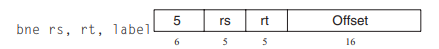
\includegraphics{413.png}
        \caption{Formato da instrução bne}
        \label{fig413}
    \end{figure}
    \begin{itemize}
        \item Ciclo de Busca: 

        A1: MAR $\leftarrow$ PC;

        A2: MBR $\leftarrow$ Memory

        PC $\leftarrow$ PC + 4;

        A3: IR $\leftarrow$ MBR;

        \item Não há ciclo indireto
        \item Ciclo de execução:

        A1: if(RS $\neq$ RT) then PC $\leftarrow$ PC + IR(offset)
    \end{itemize}
\end{itemize}

\section{Instrução lw \$t1, n}
\begin{figure}[h]
    \centering
    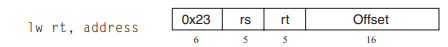
\includegraphics{42.png}
    \caption{Formato da instrução lw}
    \label{fig42}
\end{figure}

\begin{itemize}
    \item Ciclo de Busca:

    A1: MAR $\leftarrow$ PC;

    A2: MBR $\leftarrow$ Memory

    PC $\leftarrow$ PC + 4

    A3: IR $\leftarrow$ MBR;

    \item Não há ciclo indireto
    \item Ciclo de Execução:

    A1: MAR $\leftarrow$ RS + IR(offset)

    A2: MBR $\leftarrow$ (Memory)

    A3: RT $\leftarrow$ (MBR)
\end{itemize}

\section{Instrução mul \$t3, \$t1, \$t1}

\begin{figure}[h]
    \centering
    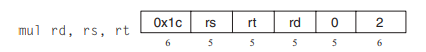
\includegraphics{43.png}
    \caption{Formato da instrução mul}
    \label{fig43}
\end{figure}

\begin{itemize}
    \item Ciclo de Busca:

    A1: MAR $\leftarrow$ PC;
    
    A2: MBR $\leftarrow$ Memory 
       
       PC $\leftarrow$ PC + 4;

    A3: IR $\leftarrow$ MBR;

    \item Não há ciclo indireto

    \item Ciclo de Execução

    A1: RD $\leftarrow$ (RS) $\times$ (RT)
\end{itemize}

\section{Instrução jal multiplication}

\begin{figure}[h]
    \centering
    
\includegraphics{44.png}
    \caption{Formato da instrução jal}
    \label{fig44}
\end{figure}

\begin{itemize}
    \item Ciclo de Busca:
    
    A1: MAR $\leftarrow$ PC;

    A2: MBR $\leftarrow$ Memory 
    
       PC $\leftarrow$ PC + 4;

    A3: IR $\leftarrow$ MBR;

    \item Não há ciclo indireto
    \item Ciclo de Execução:
    
    A1: RA $\leftarrow$ PC
    
    A2: PC $\leftarrow$ {PC[31:28], IR(target) $\times$ 4} //concatenação
\end{itemize}

\section{Instrução li \$s0, 0}

\textit{li} (Load Immediate) é uma pseudoinstrução, ou seja, não é uma instrução nativa do repertório do MIPS. Assim, é feita a tradução do \textit{li} para \textit{addiu} (Add Immediate Unsigned) ou para \textit{lui} (Load Upper Immediate) e \textit{ori} (OR Immediate), quando o valor imediato é de 16 bits ou 32 bits, respectivamente. Nesse caso, foi passado um valor de 16 bits, então haverá a execução da instrução \textit{addiu} para realizar a funcionalidade do \textit{li}.

\section{Instrução la \$a0, m1}

\textit{la} (Load Address) é uma pseudoinstrução, ou seja, não é uma instrução nativa da arquitetura MIPS. Nesse sentido, se o endereço pode ser representado um número dentro de 16 bits, é utilizado a instrução \textit{addi} (Add Immediate), caso contrário é usado as instruções \textit{lui} (Load Upper Immediate) e \textit{ori} (OR Immediate).

Para a primeira alternativa, temos:

\begin{figure}[h]
    \centering
    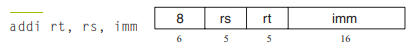
\includegraphics{461.png}
    \caption{Formato da instrução addi}
    \label{fig461}
\end{figure}

\begin{itemize}
    \item Ciclo de Busca:
    
    A1: MAR $\leftarrow$ PC;

    A2: MBR $\leftarrow$ Memory 
    
       PC $\leftarrow$ PC + 4;
    
    A3: IR $\leftarrow$ MBR;
    
    \item Não há ciclo indireto
    \item Ciclo de Execução:
    
    A1: RT $\leftarrow$ (RS) + IR(imm);
\end{itemize}

Para a segunda alternatica, temos:

\begin{figure}[h]
    \centering
    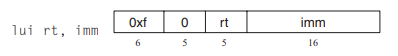
\includegraphics{462.png}
    \caption{Formato da instrução lui}
    \label{fig462}
\end{figure}

\begin{itemize}
    \item Ciclo de Busca:

    A1: MAR $\leftarrow$ PC;

    A2: MBR $\leftarrow$ Memory 
    
       PC $\leftarrow$ PC + 4;

    A3: IR $\leftarrow$ MBR;
    
    \item Não há ciclo indireto
    \item Ciclo de Execução:

    A1: ALUOut $\leftarrow$ IR(imm) << 16; //Coloca 16 bits zeros

    A2: RT $\leftarrow$ ALUOut;

\end{itemize}

\begin{figure}[h]
    \centering
    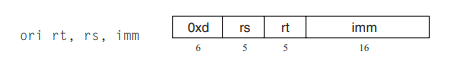
\includegraphics{463.png}
    \caption{Formato da instrução ori}
    \label{fig463}
\end{figure}

\begin{itemize}
    \item Ciclo de Busca:
    
    A1: MAR $\leftarrow$ PC;

    A2: MBR $\leftarrow$ Memory 
    
       PC $\leftarrow$ PC + 4;

    A3: IR $\leftarrow$ MBR;

    \item Não há ciclo indireto
    \item Ciclo de Execução:

    A1: IMM $\leftarrow$ ZeroExtend(IR(imm)); //Estende com zeros
    
    A2: ALUOut $\leftarrow$ RS | IMM;
    
    A3: RT $\leftarrow$ ALUOut;
\end{itemize}

\section{Instrução addu \$t6, \$a0, \$t5}

\begin{figure}[h]
    \centering
    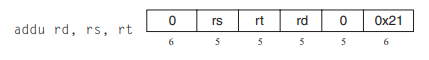
\includegraphics{47.png}
    \caption{Formato da instrução addu}
    \label{fig47}
\end{figure}

\begin{itemize}
    \item Ciclo de Busca:

    A1: MAR $\leftarrow$ PC;
    
    A2: MBR $\leftarrow$ Memory 
    
       PC $\leftarrow$ PC + 4;

    A3: IR $\leftarrow$ MBR;

    \item Não há ciclo indireto
    \item Ciclo de Execução:

    A1: RD $\leftarrow$ (RS) + (RT)
\end{itemize}

\section{Instrução l.d \$f12, (\$t6)}

Primeiramente, na arquitetura MIPS, os números de pontos flutuantes com precisão dupla são representados por 64 bits. Nesse sentido, deve-se armazenar os 32 bits mais significativos em um registrador e o restante em outro, pois os registradores suportam apenas 32 bits. Então, a pseudoinstrução l.d é convertida em dois lw (Load Word), onde f2 armazenará os bits mais significativos e f3 conterá os menos significativos. Dessa forma, executar l.d $f2, ($t6) é equivalente a realizar as instruções lw $f2, 0($t6) e lw $f3, 4($t6), para pegar os 32 bits mais significativos e menos significativos, respectivamente.

\begin{itemize}
    \item lw \$f12, 0(\$t6)
        \begin{figure}[h]
            \centering
            
\includegraphics{481.png}
            \caption{Formato da instrução lw}
            \label{fig481}
        \end{figure}

        \begin{itemize}
            \item Ciclo de Busca:
    
                A1: MAR $\leftarrow$ PC;
    
                A2: MBR $\leftarrow$ Memory 
    
                PC $\leftarrow$ PC + 4;

                A3: IR $\leftarrow$ MBR;

            \item Não há ciclo indireto
            \item Ciclo de Execução:

                A1: MAR $\leftarrow$ RS +IR(offset)

                A2: MBR $\leftarrow$ (Memory)

                A3: RT $\leftarrow$ (MBR)
        \end{itemize}

    \item lw \$f3, 4(\$t6)
        \begin{figure}[h]
            \centering
            
\includegraphics{482.png}
            \caption{Formato da instrução lw}
            \label{fig482}
        \end{figure}

        \begin{itemize}
            \item Ciclo de Busca:
                
                A1: MAR $\leftarrow$ PC;
                
                A2: MBR $\leftarrow$ Memory 
                
                    PC $\leftarrow$ PC + 4;
                
                A3: IR $\leftarrow$ MBR;

            \item Não há ciclo indireto
            \item Ciclo de Execução:

                A1: MAR $\leftarrow$ RS +IR(offset)
                
                A2: MBR $\leftarrow$ (Memory)
                
                A3: RT $\leftarrow$ (MBR)
        \end{itemize}
\end{itemize}

\section{Instrução add.d \$f2, \$f2, \$f4}

\begin{figure}[h]
    \centering
    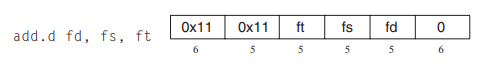
\includegraphics[width=13cm]{49.png}
    \caption{Formado da instrução add.d}
    \label{fig49}
\end{figure}

\begin{itemize}
    \item Ciclo de Busca:

    A1: MAR $\leftarrow$ PC

    A2: MBR $\leftarrow$ Memory

    PC  $\leftarrow$ PC + 4

    A3: IR  $\leftarrow$ MBR

    \item Não há ciclo indireto
    \item Ciclo de Execução:

    FPR[fd] $\leftarrow$ FPR[fs] + FPR[ft]

\end{itemize}

\section{Instrução s.d \$f2, (\$t6)}

\begin{figure}[h]
    \centering
    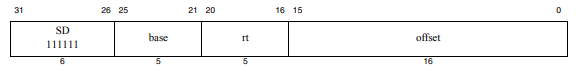
\includegraphics[width=1\linewidth]{48.png}
    \caption{Formato da instrução s.d}
    \label{fig48}
\end{figure}

\begin{itemize}
    \item Ciclo de Busca:

    A1: MAR $\leftarrow$ PC

    A2: MBR $\leftarrow$ Memory

    PC  $\leftarrow$ PC + 4

    A3: IR  $\leftarrow$ MBR

    \item Não há ciclo indireto
    \item Ciclo de Execução:

     Memória[GPR[base] $+$ offset] $\leftarrow$ GPR[rt]
     
\end{itemize}

\section{Instrução addi \$s0, \$s0, 1}

\begin{figure}[h]
    \centering
    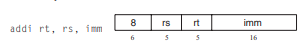
\includegraphics{4_10.png}
    \caption{Formato da instrução addi}
    \label{fig4_10}
\end{figure}

\begin{itemize}
    \item Ciclo de Busca:

    A1: MBR $\leftarrow$ PC

    A2: PC $\leftarrow$ Memory

    PC $\leftarrow$ PC + 4

    A3: IR $\leftarrow$ MBR

    \item Não há ciclo indireto

    \item Ciclo de execução:
    
    RT $\leftarrow$ RS + IMM
\end{itemize}

\section{Instrução j end}

\begin{figure}[h]
    \centering
    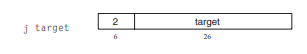
\includegraphics{4_11.png}
    \caption{Formato da instrução j}
    \label{fig4_11}
\end{figure}

\begin{itemize}
    \item Ciclo de Busca:

    A1: MBR $\leftarrow$ PC

    A2: PC $\leftarrow$ Memory

    PC $\leftarrow$ PC + 4

    A3: IR $\leftarrow$ MBR
    
    \item Não há ciclo indireto
    \item Ciclo de Execução:

    I:
    
    I+1: PC $\leftarrow$ $\text{PC}_{\text{GPRLEN-1..28}}$ \| instr\_index \| $0^2$
\end{itemize}

\section{Instrução sw \$ra, (\$sp)}

\begin{figure}[h]
    \centering
    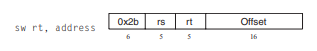
\includegraphics{4_12.png}
    \caption{Formato da instrução sw}
    \label{fig4_12}
\end{figure}

\begin{itemize}
    \item Ciclo de Busca:

    A1: MBR $\leftarrow$ PC

    A2: PC $\leftarrow$ Memory

    PC $\leftarrow$ PC + 4

    A3: IR $\leftarrow$ MBR
    \item Não há ciclo indireto
    \item Ciclo de Execução:
    
    Memória[GPR[base] + offset] $\leftarrow$ GPR[rt]
    
\end{itemize}

\section{Instrução syscall}

\begin{figure}[h]
    \centering
    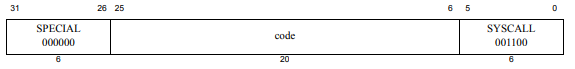
\includegraphics[width=1\linewidth]{4_13.png}
    \caption{Formato da instrução syscall}
    \label{fig4_13}
\end{figure}

\begin{itemize}
    \item Ciclo de Busca:

    A1: MBR $\leftarrow$ PC

    A2: PC $\leftarrow$ Memory

    PC $\leftarrow$ PC + 4

    A3: IR $\leftarrow$ MBR

    \item Não há ciclo indireto
    \item O ciclo de execução do syscall depende o código passado, pois essa função executa diferentes funções de acordo com o código recebido. 
    
\end{itemize}

\section{Instrução jr \$ra}

\begin{figure}[h]
    \centering
    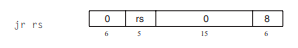
\includegraphics{4_14.png}
    \caption{Formato da instrução jr}
    \label{fig4_14}
\end{figure}

\begin{itemize}
    \item Ciclo de Busca:

    A1: MBR $\leftarrow$ PC

    A2: PC $\leftarrow$ Memory

    PC $\leftarrow$ PC + 4

    A3: IR $\leftarrow$ MBR

    \item Não há ciclo indireto
    \item Ciclo de Execução:
    
    PC $\leftarrow$ GPR[rs]
\end{itemize}

\section{Instrução move \$t4, \$v0}

Move é uma pseudoinstrução que, nesse caso, executa a função \textit{MFC0 \$t4, \$v0}.

\begin{figure}[h]
    \centering
    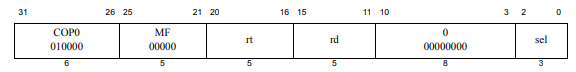
\includegraphics[width=1\linewidth]{4_15.png}
    \caption{Formato da instrução MFC0}
    \label{fig4_15}
\end{figure}

\begin{itemize}
    \item Ciclo de Busca:

    A1: MBR $\leftarrow$ PC

    A2: PC $\leftarrow$ Memory

    PC $\leftarrow$ PC + 4

    A3: IR $\leftarrow$ MBR
    \item Não há ciclo indireto.
    \item Ciclo de execução:

     GPR[rt] $\leftarrow$ CPR[0,rd,0]
\end{itemize}

\section{Instrução mul.d \$f2, \$f2, \$f4}

\begin{figure}[h]
    \centering
    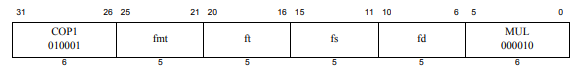
\includegraphics[width=1\linewidth]{4_16.png}
    \caption{Formato da instrução mul.d}
    \label{fig4_16}
\end{figure}

\begin{itemize}
    \item Ciclo de Busca:

    A1: MBR $\leftarrow$ PC

    A2: PC $\leftarrow$ Memory

    PC $\leftarrow$ PC + 4

    A3: IR $\leftarrow$ MBR

    \item Não há ciclo indireto
    \item Ciclo de Execução:

    FPR[fd] $\leftarrow$ FPR[fs] $\times$ FPR[ft]
\end{itemize}

% ----------------------------------------------------------
% ELEMENTOS PÓS-TEXTUAIS
% ----------------------------------------------------------
\postextual
% ----------------------------------------------------------

% ----------------------------------------------------------
% Referências bibliográficas
% ----------------------------------------------------------

\bibliography{referencias}

\nocite{a2016_mips}
\nocite{craveiro_2024_lista}
\nocite{guia}
\nocite{hennessy_2014_organizao}
\nocite{infraestrutura}
\nocite{kim_2013_the}
\nocite{missouristateuniversity_mars}
\nocite{mutlu_design}
\nocite{tabela}
\nocite{the}

\end{document}
